
\documentclass[12pt]{article}

\usepackage{amsmath, mathtools}
\usepackage{amsfonts}
\usepackage{amssymb}
\usepackage{graphicx}
\usepackage{colortbl}
\usepackage{xr}
\usepackage{hyperref}
\usepackage{longtable}
\usepackage{xfrac}
\usepackage{tabularx}
\usepackage{float}
\usepackage{siunitx}
\usepackage{booktabs}
\usepackage{caption}
\usepackage{pdflscape}
\usepackage{afterpage}

\usepackage[round]{natbib}

%\usepackage{refcheck}

\hypersetup{
    bookmarks=true,         % show bookmarks bar?
      colorlinks=true,       % false: boxed links; true: colored links
    linkcolor=red,          % color of internal links (change box color with linkbordercolor)
    citecolor=green,        % color of links to bibliography
    filecolor=magenta,      % color of file links
    urlcolor=cyan           % color of external links
}

% For easy change of table widths
\newcommand{\colZwidth}{1.0\textwidth}
\newcommand{\colAwidth}{0.13\textwidth}
\newcommand{\colBwidth}{0.82\textwidth}
\newcommand{\colCwidth}{0.1\textwidth}
\newcommand{\colDwidth}{0.05\textwidth}
\newcommand{\colEwidth}{0.8\textwidth}
\newcommand{\colFwidth}{0.17\textwidth}
\newcommand{\colGwidth}{0.5\textwidth}
\newcommand{\colHwidth}{0.28\textwidth}

% Used so that cross-references have a meaningful prefix
\newcounter{defnum} %Definition Number
\newcommand{\dthedefnum}{GD\thedefnum}
\newcommand{\dref}[1]{GD\ref{#1}}
\newcounter{datadefnum} %Datadefinition Number
\newcommand{\ddthedatadefnum}{DD\thedatadefnum}
\newcommand{\ddref}[1]{DD\ref{#1}}
\newcounter{theorynum} %Theory Number
\newcommand{\tthetheorynum}{T\thetheorynum}
\newcommand{\tref}[1]{T\ref{#1}}
\newcounter{tablenum} %Table Number
\newcommand{\tbthetablenum}{T\thetablenum}
\newcommand{\tbref}[1]{TB\ref{#1}}
\newcounter{assumpnum} %Assumption Number
\newcommand{\atheassumpnum}{P\theassumpnum}
\newcommand{\aref}[1]{A\ref{#1}}
\newcounter{goalnum} %Goal Number
\newcommand{\gthegoalnum}{P\thegoalnum}
\newcommand{\gsref}[1]{GS\ref{#1}}
\newcounter{instnum} %Instance Number
\newcommand{\itheinstnum}{IM\theinstnum}
\newcommand{\iref}[1]{IM\ref{#1}}
\newcounter{reqnum} %Requirement Number
\newcommand{\rthereqnum}{P\thereqnum}
\newcommand{\rref}[1]{R\ref{#1}}
\newcounter{nfrnum} %NFR Number
\newcommand{\rthenfrnum}{NFR\thenfrnum}
\newcommand{\nfrref}[1]{NFR\ref{#1}}
\newcounter{lcnum} %Likely change number
\newcommand{\lthelcnum}{LC\thelcnum}
\newcommand{\lcref}[1]{LC\ref{#1}}

\usepackage{fullpage}

\newcommand{\deftheory}[9][Not Applicable]
{
\newpage
\noindent \rule{\textwidth}{0.5mm}

\paragraph{RefName: } \textbf{#2} \phantomsection 
\label{#2}

\paragraph{Label:} #3

\noindent \rule{\textwidth}{0.5mm}

\paragraph{Equation:}

#4

\paragraph{Description:}

#5

\paragraph{Notes:}

#6

\paragraph{Source:}

#7

\paragraph{Ref.\ By:}

#8

\paragraph{Preconditions for \hyperref[#2]{#2}:}
\label{#2_precond}

#9

\paragraph{Derivation for \hyperref[#2]{#2}:}
\label{#2_deriv}

#1

\noindent \rule{\textwidth}{0.5mm}

}

\begin{document}


\title{Software Requirements Specification for Solar Cooker Energy Calculation: A Software for calculating heat loss and observed heat} 
\author{Deesha Patel}
\date{\today}
	
\maketitle

~\newpage

\pagenumbering{roman}

\tableofcontents

~\newpage

\section*{Revision History}

\begin{tabularx}{\textwidth}{p{3cm}p{2cm}X}
\toprule {\bf Date} & {\bf Version} & {\bf Notes}\\
\midrule
01/22/2023 & 1.0 & Initial Release\\

\bottomrule
\end{tabularx}

~\newpage

\section{Reference Material}

This section records information for easy reference.

\subsection{Table of Units}

Throughout this document SI (Syst\`{e}me International d'Unit\'{e}s) is employed
as the unit system.  In addition to the basic units, several derived units are
used as described below.  For each unit, the symbol is given followed by a
description of the unit and the SI name.
~\newline

\renewcommand{\arraystretch}{1.2}
%\begin{table}[ht]
  \noindent \begin{tabular}{l l l} 
    \toprule		
    \textbf{symbol} & \textbf{unit} & \textbf{SI}\\
    \midrule 
    \si{\metre} & length & metre\\
    \si{\kilogram} & mass	& kilogram\\
    \si{\second} & time & second\\
    \si{\celsius} & temperature & centigrade\\
    \si{\joule} & energy & joule\\
    \si{\watt} & power & watt (W = \si{\joule\per\second})\\
    \bottomrule
  \end{tabular}
  %	\caption{Provide a caption}
%\end{table}


\plt{Derived units, like newtons, pascal, etc, should show their derivation
    (the units they are derived from) if their constituent units are in the
    table of units (that is, if the units they are derived from are used in the
    document).  For instance, the derivation of pascals as
    $\si{\pascal}=\si{\newton\per\square\meter}$ is shown if newtons and m are
    both in the table.  The derivations of newtons would not be shown if kg and
    s are not both in the table.}

The symbol for units named after people use capital letters, but the name
  of the unit itself uses lower case.  For instance, pascals use the symbol Pa,
  watts use the symbol W, teslas use the symbol T, newtons use the symbol N,
  etc.  The one exception to this is degree Celsius.  Details on writing metric
  units can be found on the 
  \href{https://www.nist.gov/pml/weights-and-measures/writing-metric-units}
  {NIST} web-page.

\subsection{Table of Symbols}

The table that follows summarizes the symbols used in this document along with
their units.  The choice of symbols was made to be consistent with the heat
transfer literature and with existing documentation for solar water heating
systems.  The symbols are listed in alphabetical order.

\renewcommand{\arraystretch}{1.2}
%\noindent \begin{tabularx}{1.0\textwidth}{l l X}
\noindent \begin{longtable*}{l l p{12cm}} \toprule
\textbf{symbol} & \textbf{unit} & \textbf{description}\\
\midrule 
$A_C$ & \si[per-mode=symbol] {\square\metre} & coil surface area
\\
$A_\text{in}$ & \si[per-mode=symbol] {\square\metre} & surface area over 
which heat is transferred in
\\ 
\bottomrule
\end{longtable*}
\plt{Use your problems actual symbols.  The si package is a good idea to use for
  units.}

\subsection{Abbreviations and Acronyms}

\renewcommand{\arraystretch}{1.2}
\begin{tabular}{l l} 
  \toprule		
  \textbf{symbol} & \textbf{description}\\
  \midrule 
  A & Assumption\\
  DD & Data Definition\\
  GD & General Definition\\
  GS & Goal Statement\\
  IM & Instance Model\\
  LC & Likely Change\\
  PS & Physical System Description\\
  R & Requirement\\
  SRS & Software Requirements Specification\\
  \progname{} & \plt{put an expanded version of your program name here (as appropriate)}\\
  T & Theoretical Model\\
  \bottomrule
\end{tabular}\\

\plt{Add any other abbreviations or acronyms that you add}

\subsection{Mathematical Notation}

\plt{This section is optional, but should be included for projects that make use
  of notation to convey mathematical information.  For instance, if typographic
  conventions (like bold face font) are used to distinguish matrices, this
  should be stated here.  If symbols are used to show mathematical operations,
  these should be summarized here.  In some cases the easiest way to summarize
  the notation is to point to a text or other source that explains the
  notation.}

\plt{This section was added to the template because some students use very
  domain specific notation.  This notation will not be readily understandable to
  people outside of your domain.  It should be explained.}

\newpage

\pagenumbering{arabic}

\plt{This SRS template is based on \citet{SmithAndLai2005, SmithEtAl2007}.  It
  will get you started.  You should not modify the section headings, without
  first discussing the change with the course instructor.  Modification means
  you are not following the template, which loses some of the advantage of a
  template, especially standardization.  Although the bits shown below do not
  include type information, you may need to add this information for your
  problem.  If you are unsure, please can ask the instructor.}

\plt{Feel free to change the appearance of the report by modifying the LaTeX
  commands.}

\plt{This template document assumes that a single program is being documented.
  If you are documenting a family of models, you should start with a commonality
  analysis.  A separate template is provided for this.  For program
  families you should look at \cite{Smith2006, SmithMcCutchanAndCarette2017}.
  Single family member programs are often programs based on a single physical
  model.  General purpose tools are usually documented as a family.  Families of
  physical models also come up.}

\plt{The SRS is not generally written, or read, sequentially.  The SRS is a
  reference document.  It is generally read in an ad hoc order, as the need
  arises.  For writing an SRS, and for reading one for the first time, the
  suggested order of sections is:
\begin{itemize}
\item Goal Statement
\item Instance Models
\item Requirements
\item Introduction
\item Specific System Description
\end{itemize}
}

\plt{Guiding principles for the SRS document:
\begin{itemize}
\item Do not repeat the same information at the same abstraction level.  If
  information is repeated, the repetition should be at a different abstraction
  level.  For instance, there will be overlap between the scope section and the
  assumptions, but the scope section will not go into as much detail as the
  assumptions section.
\end{itemize}
}

\plt{The template description comments should be disabled before submitting this
  document for grading.}

\plt{You can borrow any wording from the text given in the template.  It is part
  of the template, and not considered an instance of academic integrity.  Of
  course, you need to cite the source of the template.}

\plt{When the documentation is done, it should be possible to trace back to the
  source of every piece of information.  Some information will come from
  external sources, like terminology.  Other information will be derived, like
  General Definitions.}

\plt{An SRS document should have the following qualities: unambiguous,
  consistent, complete, validatable, abstract and traceable.}

\plt{The overall goal of the SRS is that someone that meets the Characteristics
  of the Intended Reader (Section~\ref{sec_IntendedReader}) can learn,
  understand and verify the captured domain knowledge.  They should not have to
  trust the authors of the SRS on any statements.  They should be able to
  independently verify/derive every statement made.}

\section{Introduction}

\plt{
As fossil fuels adversely affect the environment, many countries like India, where they have good Solar rays throughout the year, have started to implement devices for utilizing solar energy and transforming it into valuable energy. It includes Solar Water heaters, Solar panels, and Solar Cookers. It is indeed a fact that the demand for renewable energy has increased to deal with the problem. Focusing on solar cooker, several design such as Solar Panel Cooker, Solar Parabolic Cooker, and Solar Box Cooker has been proposed to utilize more solar energy. Using internal reflectors, we would like to improve the utilization of solar energy during cooking a food.   

The following section provides an overview of Software Requirement Specification (SRS) for a box-type Solar Cooker. This section explains the purpose of the document, the scope of requirements, the characteristic of the intended reader, and the organization of a document.   

}

\subsection{Purpose of Document}

We are going to use the Solar Box Cooker in this software. The main purpose of this document is to describe a mathematical model of a Solar Cooker which can provide a calculation for internal reflector in solar box that can help to improve the temperature in the box. It includes a variety of parameters that attempts to define the intended functionality required. Thus, this document provides detailed requirements of the software which will be used in planing for design stage. Therefore, this document is intended to be used as a reference to provide ad hoc access to all information necessary to understand and verify the model. This document describes goals, assumptions, theoretical models, and important definitions to understand the problem. The SRS is abstract because the content here says \emph{what} the problem is. But it does not say anything related to \emph{how} to solve it.

This document will be used as a starting point for subsequent development 
phases, including writing the design specification and the software 
verification and validation plan. The design document will show how the 
requirements are to be realized, including decisions on the numerical 
algorithms and programming environment. The verification and validation plan 
will show the steps that will be used to increase confidence in the software 
documentation and the implementation. Although the SRS fits in a series of 
documents that follow the so-called waterfall model, the actual development 
process is not constrained in any way. Even when the waterfall model is not 
followed, as Parnas and Clements~\cite{ParnasAndClements} point out, the most logical way to 
present the documentation is still to “fake” a rational design process.

\subsection{Scope of Requirements} 

There are Numerous algorithm has been proposed to improve the efficiency of Solar Cooker. The scope of the requirement includes a mathematical model to determine the thermal function of a box-type solar cooker with an internal reflectors. With the help of different inputs, this system calculates the achieved temperature by implementing the proposed solution. However, this project not focusing on more than one iteration for the reflections. 

\subsection{Characteristics of Intended Reader} \label{sec_IntendedReader}

Firstly, Intended Reader or Reviewer should have knowledge of heat transfer theory and radiant solar energy. A person should have completed a Heat Transfer course during their bachelor of engineering (Mechanical Engineering expected). A reader should have knowledge about the coupled differential equation; offered in the Calculus course.        

\subsection{Organization of Document}

The organization of this document follows the template for an SRS for scientific 
computing software proposed by~\cite{Koothoor2013} and \cite{SmithAndLai2005}.
The presentation follows the standard pattern of presenting goals, theories, definitions, 
and assumptions. For readers that would like a more bottom up approach, they can start 
reading the instance models in Section~\ref{sec_instance} and trace back to find any 
additional information they require. The goal statements are refined to the theoretical models, 
and the theoretical models to the instance models. The instance model 
(Section~\ref{sec_instance}) to be solved is referred to as \iref{ewat}. The instance model provides 
the Ordinary Differential Equation (ODE) that model the solar water heating system. 
SWHS solves this ODE.

\section{General System Description}

This section provides general information about the system.  It identifies the
interfaces between the system and its environment, describes the user
characteristics and lists the system constraints.  

\subsection{System Context}

The system context is shown in Figure \ref{Fig_SystemContext} below. The circles represent the user, who is both responsible for handling the inputs and the outputs. The box represents the program itself, and the arrows indicate what data and information is passed from the user to the program. 

\begin{figure}[h!]
\begin{center}
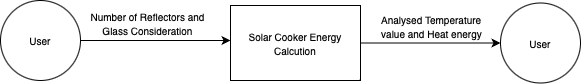
\includegraphics[width=0.6\textwidth]{SystemContext}
\caption{System Context}
\label{Fig_SystemContext} 
\end{center}
\end{figure}

\begin{itemize}
\item User Responsibilities:
\begin{itemize}
\item Provide required inputs including number of reflectors, glass area, thickness, dimension and size. 
\item Ensure all inputs are in correct format. 
\end{itemize}

\item Responsibilities:
\begin{itemize}
\item Detect data type mismatch, such as a string of characters instead of a
  floating point number
\item Determine if the inputs satisfy the required physical and software constraints such as thickness of the glass can not be a negative value
\item Calculate and plot the required outputs of temperature
\end{itemize}
\end{itemize}

\subsection{User Characteristics} \label{SecUserCharacteristics}

The end user of the system is expected to be familiar with Undergraduate level Calculus and basic physics. They should also know basics about the Reflector angle and heat flows in solar cooker.  

\subsection{System Constraints}

There are no system constraints for this project.

\section{Specific System Description}

This section first presents the problem description, which gives a high-level
view of the problem to be solved.  This is followed by the solution characteristics
specification, which presents the assumptions, theories, definitions and finally
the instance models (ODE) that models the Solar Cooker Reflections.

\subsection{Problem Description} \label{Sec_pd}

Solar Cooker Energy Calculation is intended to investigate the temperature inside the solar cooker box with internal reflectors. 

\subsubsection{Terminology and  Definitions}

This subsection provides a list of terms that are used in the subsequent
sections and their meaning, with the purpose of reducing ambiguity and making it
easier to correctly understand the requirements:

\begin{itemize}

\item Reflectivity: The fraction of radiation reflected by the surface is called the reflectivity ($\rho$) 
\item Absorptivity: The fraction of irradiation absorbed by the surface is called the absorptivity ($\alpha$)
\item Transmittivity: The fraction of radiation transmitted is called the transmissivity ($\tau$)
\item Emittance: the energy radiated by the surface of a body per second per unit area ($\epsilon$)
\item Reflactor Angle: the angle between a reflected ray and the normal drawn at the point of incidence to a reflecting surface ($\theta$)
\item Heat flow Convection: Convection is the transfer of heat from one place to another due to the movement of fluid 
\item Heat flow radiation: a process where heat waves are emitted that may be absorbed, reflected, or transmitted through a colder body
\item Heat Convection Coefficients: The rate of heat transfer between a solid surface and a fluid per unit surface area per unit temperature difference (h) 
\item Steffan-Boltzman constant: is a physical constant expressing the relationship between the heat radiation emitted by a black body and its absolute temperature ($\sigma$)
\item Heat Flux: the amount of heat energy passing through a certain surface


\end{itemize}

\subsubsection{Physical System Description} \label{sec_phySystDescrip}

The physical system of Solar Cooker
Energy Calculation, as shown in Figure \ref{Fig_HeatFlows},
includes the following elements:


\begin{itemize}

\item[PS1:] A cover with two flat glasses (glass 1 and glass 2) 

\item[PS2:] Lead of the recipient and recipient itself

\item[PS3:] Fluid inside the recipient

\end{itemize}

\begin{figure}[h!]
\begin{center}
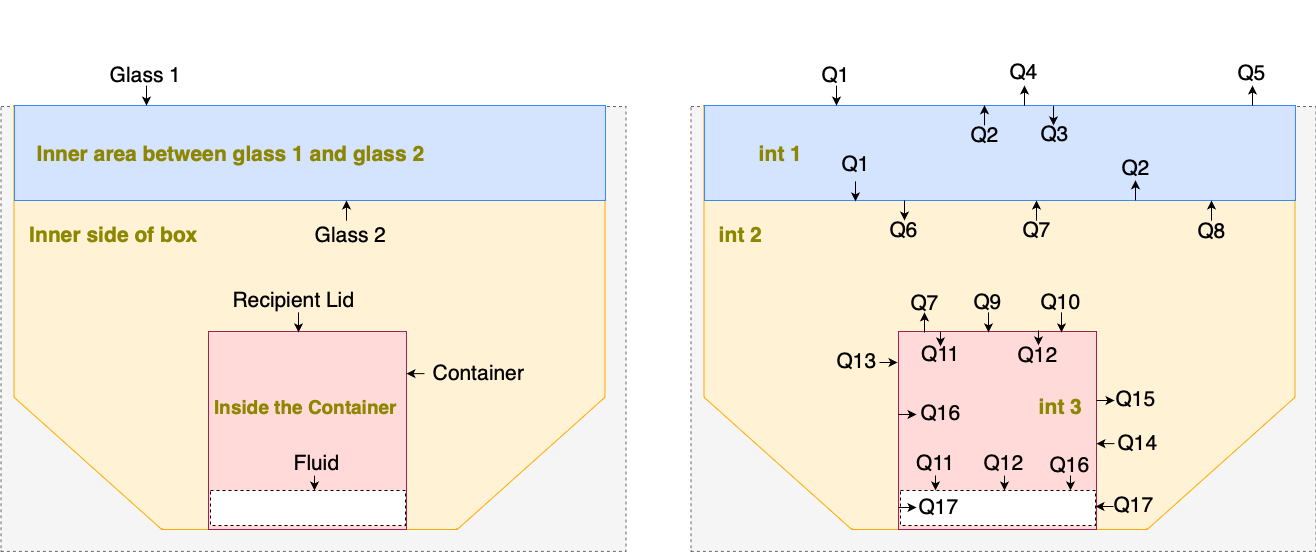
\includegraphics[width=0.45\textwidth]{HeatFlow}
\caption{Heat Flows in Solar Cooker}
\label{Fig_HeatFlows} 
\end{center}
\end{figure}


% \begin{figure}[h!]
% \begin{center}
% %\rotatebox{-90}
% {
%  \includegraphics[width=0.5\textwidth]{<FigureName>}
% }
% \caption{\label{<Label>} <Caption>}
% \end{center}
% \end{figure}

\subsubsection{Goal Statements}

\noindent Given the Area of glass, Incident solar radiation, difference in temperature, Reflection angle, Steffan-Boltzman constant, heat transfer convection coefficient, the goal statements are:

\begin{itemize}

\item[GS\refstepcounter{goalnum}\thegoalnum \label{G_meaningfulLabel}:] \plt{predicts the Balance of energy in the recipient.}

\item[GS\refstepcounter{goalnum}\thegoalnum \label{G_meaningfulLabel}:] \plt{predicts the cooking power in the recipient.}

\end{itemize}

\subsection{Solution Characteristics Specification}

The instance model (ODE) that governs Solar Cooker
Energy Calculation is presented in
Subsection~\ref{sec_instance}.  The information to understand the meaning of the
instance model and its derivation is also presented, so that the instance
model can be verified.

\subsubsection{Assumptions} \label{sec_assumpt}


This section simplifies the original problem and helps in developing the
theoretical model by filling in the missing information for the physical
system. The numbers given in the square brackets refer to the theoretical model
[T], general definition [GD], data definition [DD], instance model [IM], or
likely change [LC], in which the respective assumption is used.

\begin{itemize}

\item[A\refstepcounter{assumpnum}\theassumpnum \label{A_common_constant}:] Properties like emissivity(\si{\epsilon}) reflectivity (\si{\rho}) and transmisivity (\si{\tau}) have been considered constant [\dref{HFC}, \iref{ewat}]

\item[A\refstepcounter{assumpnum}\theassumpnum \label{A_fluid_type}:] The material in the recipient (Container) is liquid for this case (For us, it's water). This implies that the  temperature will not drop below melting point and not rise above the boiling point [\iref{ewat}, \tref{T:SHE}]   

\item[A\refstepcounter{assumpnum}\theassumpnum \label{A_int_temp_formula}:] The temperature $T_\text{int2}$ are obtained in function of others temperatures by means of the following supposition: [\iref{ewat}] 
~\newline
\begin{center}  
$T_\text{int2} = \frac{T_\text{g2} + T_t + T_r}{3} $ 
\end{center}

\item[A\refstepcounter{assumpnum}\theassumpnum \label{A_radiation_impact}:] The solar radiation impact over the solar cooker occurs in perpendicular way. [\iref{ewat}] 

\end{itemize}

\subsubsection{Theoretical Models}\label{sec_theoretical}

This section focuses on the general equations and laws that Solar Cooker
Energy Calculation is based
on. Theoretical models are sets of abstract mathematical equations or axioms
  for solving the problem described in Section ``Physical System Description''
  (Section~\ref{sec_phySystDescrip}). Examples of theoretical models are
  physical laws, constitutive equations, relevant conversion factors, etc.



~\newline

\noindent
\deftheory
% #2 refname of theory
{T:CHTC}
% #3 label
{Convective Heat Transfer Coefficient}
% #4 equation
{
  h = $\frac{q}{\triangle T}$
}
% #5 description
{
  The above equation is used to calculate the heat transfer typically by convection or phase transition. ~\newline
  
  h is the heat transfer convection coefficient (\si[per-mode=symbol] {\watt\per\square\metre} K). ~\newline 
  
  q is the thermal flux vector (\si{\watt\per\square\metre} ). ~\newline 
  
  $\triangle$T is the change in temperature.
}
% #6 Notes
{
None.
}
% #7 Source
{
  \url{https://en.wikipedia.org/wiki/Heat_transfer_coefficient}
}
% #8 Referenced by
{
  \dref{HFC}, \iref{ewat}
}
% #9 Preconditions
{
None
}
% #1 derivation - not applicable by default
{}


~\newline


\noindent
\deftheory
% #2 refname of theory
{T:SHE}
% #3 label
{Sensible Heat energy Calculation}
% #4 equation
{
  Q = $Cm \triangle T$
}
% #5 description
{
  This calculation occurs until the highest or lowest temperature reach, as assumed in [\aref{A_fluid_type}] ~\newline
  Q is the quantity of heat transferred to or from the object ~\newline 
  m is the mass of the object ~\newline 
  C is the specific heat capacity of the material the object is composed of ~\newline 
  \si{\triangle} T is the resulting temperature change of the object ~\newline 
}
% #6 Notes
{
None.
}
% #7 Source
{
  \url{https://www.physicsclassroom.com/class/thermalP/Lesson-2/Measuring-the-Quantity-of-Heat}
}
% #8 Referenced by
{
  \iref{ewat}
}
% #9 Preconditions
{
None
}
% #1 derivation - not applicable by default
{}


~\newline


\subsubsection{General Definitions}\label{sec_gendef}

\plt{General Definitions (GDs) are a refinement of one or more TMs, and/or of
  other GDs.  The GDs are less abstract than the TMs.  Generally the reduction
  in abstraction is possible through invoking (using/referencing) Assumptions.
  For instance, the TM could be Newton's Law of Cooling stated abstracting.  The
  GD could take the general law and apply it to get a 1D equation.}

This section collects the laws and equations that will be used in building the
instance models.

\plt{Some projects may not have any content for this section, but the section
  heading should be kept.}  \plt{Modify the examples below for your problem, and
  add additional definitions as appropriate.}

~\newline

\noindent
\begin{minipage}{\textwidth}
\renewcommand*{\arraystretch}{1.5}
\begin{tabular}{| p{\colAwidth} | p{\colBwidth}|}
\hline
\rowcolor[gray]{0.9}
Number& GD\refstepcounter{defnum}\thedefnum \label{HFC}\\
\hline
Label &\bf Heat Flow Convection \\
\hline
% Units&$MLt^{-3}T^0$\\
% \hline
SI Units&\si{\watt}\\
\hline
Equation&$ Q(t) = hA \Delta T(t)$  \\
\hline
Description &
Heat Flow Convection is related to Newton's law of cooling describes convective cooling from a surface.  The law is
stated as: the rate of heat loss from a body is proportional to the difference
in temperatures between the body and its surroundings.
\\
& $Q(t)$ is the thermal flux (\si{\watt\per\square\metre}).\\
& $h$ is the heat transfer coefficient
	(\si{\watt\per\square\metre\per\celsius}).\\
 & $A$ is the exposed surface area (\si[per-mode=symbol] {\square\metre}). \\  
&$\Delta T(t)$ is the time-difference (\si{\celsius}).
\\
\hline
  Source & \url{https://en.wikipedia.org/wiki/Convection_(heat_transfer)} \\
  \hline
  Ref.\ By & \iref{ewat}\\
  \hline
\end{tabular}
\end{minipage}\\


~\newline

\noindent
\begin{minipage}{\textwidth}
\renewcommand*{\arraystretch}{1.5}
\begin{tabular}{| p{\colAwidth} | p{\colBwidth}|}
\hline
\rowcolor[gray]{0.9}
Number& GD\refstepcounter{defnum}\thedefnum \label{HFC}\\
\hline
Label &\bf Heat Flow Radiation \\
\hline
% Units&$MLt^{-3}T^0$\\
% \hline
SI Units&\si{\joule}\\
\hline
Equation&$ Q(t) = \sigma eA \triangle T^4$  \\
\hline
Description &
An object emits radiant energy in all directions unless its temperature is absolute zero. If this energy strikes a receiver, part of it may be absorbed, part may be transmitted, and part may be reflected. Heat transfer from a hot to a cold object in this manner is known as radiation heat transfer . The higher the temperature, the greater is the amount of energy radiated.
\\
& $Q(t)$ is the heat flow radiation (\si{\watt\per\square\metre}).\\
& $\sigma$ is the Steffan-Boltzman constant
	$(5.669 X 10^{-8} W / m^2 K^4)$.\\
 & $e$ is the emissivity of object(\si[per-mode=symbol] {\watt\per\metre}). \\  
 & $A$ is the exposed surface area (\si[per-mode=symbol] {\square\metre}) \\
&$\triangle T(t)$ is the time-difference (\si{\celsius}).
\\
\hline
  Source & ~\cite{rediationdef} \\
  \hline
  Ref.\ By & \iref{ewat}\\
  \hline
\end{tabular}
\end{minipage}\\


~\newline


\subsubsection*{Detailed derivation of simplified rate of change of temperature}

\plt{This may be necessary when the necessary information does not fit in the
  description field.}
\plt{Derivations are important for justifying a given GD.  You want it to be
  clear where the equation came from.}

\subsubsection{Data Definitions}\label{sec_datadef}

\plt{The Data Definitions are definitions of symbols and equations that are
  given for the problem.  They are not derived; they are simply used by other
  models.  For instance, if a problem depends on density, there may be a data
  definition for the equation defining density.  The DDs are given information
  that you can use in your other modules.}

\plt{All Data Definitions should be used (referenced) by at least one other
  model.}

This section collects and defines all the data needed to build the instance
models. The dimension of each quantity is also given.  \plt{Modify the examples
  below for your problem, and add additional definitions as appropriate.}

~\newline

\noindent
\begin{minipage}{\textwidth}
\renewcommand*{\arraystretch}{1.5}
\begin{tabular}{| p{\colAwidth} | p{\colBwidth}|}
\hline
\rowcolor[gray]{0.9}
Number& DD\refstepcounter{datadefnum}\thedatadefnum \label{FluxCoil}\\
\hline
Label& \bf Heat flux over all different object\\
\hline
Symbol &$q$\\
\hline
% Units& $Mt^{-3}$\\
% \hline
  SI Units & \si{\watt\per\square\metre}\\
  \hline
  Equation&$q (t) = -\lambda \frac{\triangle T}{\triangle x} \\
  \hline
  Description & It is necessary to know the thermal conductivity of a material if you want to calculate the heat energy transferred through it \\
  
  &$q$ is the heat flux  \\
               &$\lambda$ is the thermal conductivity of the material \\ 
                &$\triangle T$ is the temperature difference across the object \\
                &$\triangle x$ is the distance of heat   transfer (the thickness of the object) 
\\
  \hline
  Sources& \url{https://www.omnicalculator.com/physics/thermal-conductivity} \\
  \hline
  Ref.\ By & \iref{ewat}\\
  \hline
\end{tabular}
\end{minipage}\\


\subsubsection{Instance Models} \label{sec_instance}    

This section transforms the problem defined in Section~\ref{Sec_pd} into 
one which is expressed in mathematical terms. It uses concrete symbols defined 
in Section~\ref{sec_datadef} to replace the abstract symbols in the models 
identified in Sections~\ref{sec_theoretical}.


~\newline

%Instance Model 1

\noindent
\begin{minipage}{\textwidth}
\renewcommand*{\arraystretch}{1.5}
\begin{tabular}{| p{\colAwidth} | p{\colBwidth}|}
  \hline
  \rowcolor[gray]{0.9}
  Number& IM\refstepcounter{instnum}\theinstnum \label{ewat}\\
  \hline
  Label& \bf Balance of energy on the recipient to find $T_r$\\
  \hline
  Input&$A_r$, $\epsilon_r$, $T_r$, $T_f$, $T_\text{int2}$, $A_m$, $T_f$\\
  & The input is constrained so that $\epsilon_t \leq 0 $ \\
  \hline
  Output&$T_f(t)$, $t \geq 0 $, such that\\

  & $ \bf m_r c_r  \frac{dT_r}{dt} $ $  = Q13 + 4Q14 - Q15 - Q16 - Q17 \\
  \hline
  Description
   & $\textbf{Q13} = A_r h_\text{r-int2}(T_\text{int2} - T_r)$ - Heat flow convection of recipient to the inner 2\\
  & $\textbf{Q14} = 4\sum_{i=1}^n \rho A_\text{ref,n} G \tau_g^2 cos (90 - \theta_\text{ref,n})$ - Heat flow reflection of incident radiation on the reflectors \\
  & $\textbf{Q15} = A_r \sigma \epsilon_r (T^4_r - T^4_\text{g2})$ - Heat flow radiation of recipient toward glass 2 \\ 
  & $\textbf{Q16} = A_r \sigma \epsilon_r (T^4_r - T^4_\text{f})$ - Heat flow radiation of recipient toward the fluid\\
  & $\textbf{Q17} = A_m h_\text{r-f}(T_r - T_f)$ - Heat flow convection of recipient toward the fluid \\
  &$A_r$ is the Area of Reflector (\si{\square\metre}).\\
  &$\epsilon_r$ is the Emittance of recipient (\si[per-mode=symbol] {\watt\per\metre}).\\
  &$T_r$ is the Reflector temperature (\si{\celsius}).\\
  &$T_\text{g2}$ is a temperature of glass 2 (\si{\celsius}).\\
  &$T_\text{int2}$ is a temperature inside the box (\si{\celsius}).\\
  &$G$ is the Incidental solar radiation (\si[per-mode=symbol] {\watt\per\square\metre}).\\
  &$T_f$ is a current temperature of Fluid (\si{\celsius}).\\
  

  & The above equation applies as long as the fluid is in liquid form,
  $0<T_f<100^o\text{C}$, where $0^o\text{C}$ and $100^o\text{C}$ are the melting
  and boiling points of water(as we are using water for testing), respectively.
  \\
  \hline
  Sources& \cite{MathsModel} \\
  \hline
  Ref.\ By & None\\
  \hline
\end{tabular}
\end{minipage}\\

~\newline

\noindent
\begin{minipage}{\textwidth}
\renewcommand*{\arraystretch}{1.5}
\begin{tabular}{| p{\colAwidth} | p{\colBwidth}|}
  \hline
  \rowcolor[gray]{0.9}
  Number& IM\refstepcounter{instnum}\theinstnum \label{I_HWAT}\\
  \hline
  Label& \bf Heat energy in the recipient\\
  \hline
  Input&$C_W$, $m_W$, $T_\text{init}$, $T_W(t)$\\
  \hline
  Output&$E_W(t)$, $0 \leq t \leq t_\text{final}$, such that\\
  &$E_W(t)$ = $C_W m_W (T_W(t) - T_\text{init})$\\
  \hline
  Description & The above equation is derived using \tref{T:SHE}.  $E_W$ is the 
  change in thermal energy of the liquid water relative to the energy at the initial 
  temperature ($T_\text{init}$).  $C_W$ is the specific heat capacity of liquid water and $m_W$ is 
  the mass of the water.  The change in temperature is the difference between 
  the temperature at time t, $T_W$, and the initial temperature, $T_\text{init}$, this
  equation applies as long as $0 < T_W < 100^o\text{C}$ (\aref{A_fluid_type}).\\
  \hline
  Sources&~\cite{Lightstone2012}\ \\
  \hline
  Ref.\ By & --\\
  \hline
\end{tabular}
\end{minipage}\\

~\newline

\subsubsection*{Derivation of ...}

\plt{The derivation shows how the IM is derived from the TMs/GDs.  In cases
  where the derivation cannot be described under the Description field, it will
  be necessary to include this subsection.}

\subsubsection{Input Data Constraints} \label{sec_DataConstraints}    

Table~\ref{TblInputVar} shows the data constraints on the input output
variables.  The column for physical constraints gives the physical limitations
on the range of values that can be taken by the variable.  The column for
software constraints restricts the range of inputs to reasonable values.  The
software constraints will be helpful in the design stage for picking suitable
algorithms.  The constraints are conservative, to give the user of the model the
flexibility to experiment with unusual situations.  The column of typical values
is intended to provide a feel for a common scenario.  The uncertainty column
provides an estimate of the confidence with which the physical quantities can be
measured.  This information would be part of the input if one were performing an
uncertainty quantification exercise.

The specification parameters in Table~\ref{TblInputVar} are listed in
Table~\ref{TblSpecParams}.

\begin{table}[!h]
  \caption{Input Variables} \label{TblInputVar}
  \renewcommand{\arraystretch}{1.2}
\noindent \begin{longtable*}{l l l l c} 
  \toprule
  \textbf{Var} & \textbf{Physical Constraints} & \textbf{Software Constraints} &
                             \textbf{Typical Value} & \textbf{Uncertainty}\\
  \midrule 
  $L$ & $L > 0$ & $L_{\text{min}} \leq L \leq L_{\text{max}}$ & 1.5 \si[per-mode=symbol] {\metre} & 10\%
  \\
  \bottomrule
\end{longtable*}
\end{table}

\noindent 
\begin{description}
\item[(*)] \plt{you might need to add some notes or clarifications}
\end{description}

\begin{table}[!h]
\caption{Specification Parameter Values} \label{TblSpecParams}
\renewcommand{\arraystretch}{1.2}
\noindent \begin{longtable*}{l l} 
  \toprule
  \textbf{Var} & \textbf{Value} \\
  \midrule 
  $L_\text{min}$ & 0.1 \si{\metre}\\
  \bottomrule
\end{longtable*}
\end{table}

\subsubsection{Properties of a Correct Solution} \label{sec_CorrectSolution}

\noindent
A correct solution must exhibit \plt{fill in the details}.  \plt{These
  properties are in addition to the stated requirements.  There is no need to
  repeat the requirements here.  These additional properties may not exist for
  every problem.  Examples include conservation laws (like conservation of
  energy or mass) and known constraints on outputs, which are usually summarized
  in tabular form.  A sample table is shown in Table~\ref{TblOutputVar}}

\begin{table}[!h]
\caption{Output Variables} \label{TblOutputVar}
\renewcommand{\arraystretch}{1.2}
\noindent \begin{longtable*}{l l} 
  \toprule
  \textbf{Var} & \textbf{Physical Constraints} \\
  \midrule 
  $T_W$ & $T_\text{init} \leq T_W \leq T_C$ (by~\aref{A_charge})
  \\
  \bottomrule
\end{longtable*}
\end{table}

\plt{This section is not for test cases or techniques for verification and
  validation.  Those topics will be addressed in the Verification and Validation
  plan.}

\section{Requirements}

\plt{The requirements refine the goal statement.  They will make heavy use of
  references to the instance models.}

This section provides the functional requirements, the business tasks that the
software is expected to complete, and the nonfunctional requirements, the
qualities that the software is expected to exhibit.

\subsection{Functional Requirements}

\noindent \begin{itemize}

\item[R\refstepcounter{reqnum}\thereqnum \label{R_Inputs}:] \plt{Requirements
    for the inputs that are supplied by the user.  This information has to be
    explicit.}

\item[R\refstepcounter{reqnum}\thereqnum \label{R_OutputInputs}:] \plt{It isn't
    always required, but often echoing the inputs as part of the output is a
    good idea.}

\item[R\refstepcounter{reqnum}\thereqnum \label{R_Calculate}:] \plt{Calculation
    related requirements.}

\item[R\refstepcounter{reqnum}\thereqnum \label{R_VerifyOutput}:]
  \plt{Verification related requirements.}

\item[R\refstepcounter{reqnum}\thereqnum \label{R_Output}:] \plt{Output related
    requirements.}

\end{itemize}

\plt{Every IM should map to at least one requirement, but not every requirement
  has to map to a corresponding IM.}

\subsection{Nonfunctional Requirements}

\plt{List your nonfunctional requirements.  You may consider using a fit
  criterion to make them verifiable.}
\plt{The goal is for the nonfunctional requirements to be unambiguous, abstract
  and verifiable.  This isn't easy to show succinctly, so a good strategy may be
to give a ``high level'' view of the requirement, but allow for the details to
be covered in the Verification and Validation document.}
\plt{An absolute requirement on a quality of the system is rarely needed.  For
  instance, an accuracy of 0.0101 \% is likely fine, even if the requirement is
  for 0.01 \% accuracy.  Therefore, the emphasis will often be more on
  describing now well the quality is achieved, through experimentation, and
  possibly theory, rather than meeting some bar that was defined a priori.}
\plt{You do not need an entry for correctness in your NFRs.  The purpose of the
  SRS is to record the requirements that need to be satisfied for correctness.
  Any statement of correctness would just be redundant. Rather than discuss
  correctness, you can characterize how far away from the correct (true)
  solution you are allowed to be.  This is discussed under accuracy.}

\noindent \begin{itemize}

\item[NFR\refstepcounter{nfrnum}\thenfrnum \label{NFR_Accuracy}:]
  \textbf{Accuracy} \plt{Characterize the accuracy by giving the context/use for
    the software.  Maybe something like, ``The accuracy of the computed
    solutions should meet the level needed for $<$engineering or scientific
    application$>$.  The level of accuracy achieved by \progname{} shall be
    described following the procedure given in Section~X of the Verification and
    Validation Plan.''  A link to the VnV plan would be a nice extra.}

\item[NFR\refstepcounter{nfrnum}\thenfrnum \label{NFR_Usability}:] \textbf{Usability}
  \plt{Characterize the usability by giving the context/use for the software.
    You should likely reference the user characteristics section.  The level of
    usability achieved by the software shall be described following the
    procedure given in Section~X of the Verification and Validation Plan.  A
    link to the VnV plan would be a nice extra.}

\item[NFR\refstepcounter{nfrnum}\thenfrnum \label{NFR_Maintainability}:]
  \textbf{Maintainability} \plt{The effort required to make any of the likely
    changes listed for \progname{} should be less than FRACTION of the original
    development time.  FRACTION is then a symbolic constant that can be defined
    at the end of the report.}

\item[NFR\refstepcounter{nfrnum}\thenfrnum \label{NFR_Portability}:]
  \textbf{Portability} \plt{This NFR is easier to write than the others.  The
    systems that \progname{} should run on should be listed here.  When possible
    the specific versions of the potential operating environments should be
    given.  To make the NFR verifiable a statement could be made that the tests
    from a given section of the VnV plan can be successfully run on all of the
    possible operating environments.}

\item Other NFRs that might be discussed include verifiability,
  understandability and reusability.

\end{itemize}

\section{Likely Changes}    

\noindent \begin{itemize}

\item[LC\refstepcounter{lcnum}\thelcnum\label{LC_meaningfulLabel}:] \plt{Give
    the likely changes, with a reference to the related assumption (aref), as appropriate.}

\end{itemize}

\section{Unlikely Changes}    

\noindent \begin{itemize}

\item[LC\refstepcounter{lcnum}\thelcnum\label{LC_meaningfulLabel}:] \plt{Give
    the unlikely changes.  The design can assume that the changes listed will
    not occur.}

\end{itemize}

\section{Traceability Matrices and Graphs}

The purpose of the traceability matrices is to provide easy references on what
has to be additionally modified if a certain component is changed.  Every time a
component is changed, the items in the column of that component that are marked
with an ``X'' may have to be modified as well.  Table~\ref{Table:trace} shows the
dependencies of theoretical models, general definitions, data definitions, and
instance models with each other. Table~\ref{Table:R_trace} shows the
dependencies of instance models, requirements, and data constraints on each
other. Table~\ref{Table:A_trace} shows the dependencies of theoretical models,
general definitions, data definitions, instance models, and likely changes on
the assumptions.

\plt{You will have to modify these tables for your problem.}

\plt{The traceability matrix is not generally symmetric.  If GD1 uses A1, that
  means that GD1's derivation or presentation requires invocation of A1.  A1
  does not use GD1.  A1 is ``used by'' GD1.}

\plt{The traceability matrix is challenging to maintain manually.  Please do
  your best.  In the future tools (like Drasil) will make this much easier.}

\afterpage{
\begin{landscape}
\begin{table}[h!]
\centering
\begin{tabular}{|c|c|c|c|c|c|c|c|c|c|c|c|c|c|c|c|c|c|c|c|}
\hline
	& \aref{A_OnlyThermalEnergy}& \aref{A_hcoeff}& \aref{A_mixed}& \aref{A_tpcm}& \aref{A_const_density}& \aref{A_const_C}& \aref{A_Newt_coil}& \aref{A_tcoil}& \aref{A_tlcoil}& \aref{A_Newt_pcm}& \aref{A_charge}& \aref{A_InitTemp}& \aref{A_OpRangePCM}& \aref{A_OpRange}& \aref{A_htank}& \aref{A_int_heat}& \aref{A_vpcm}& \aref{A_PCM_state}& \aref{A_Pressure} \\
\hline
\tref{T_COE}        & X& & & & & & & & & & & & & & & & & & \\ \hline
\tref{T_SHE}        & & & & & & & & & & & & & & & & & & & \\ \hline
\tref{T_LHE}        & & & & & & & & & & & & & & & & & & & \\ \hline
\dref{NL}           & & X& & & & & & & & & & & & & & & & & \\ \hline
\dref{ROCT}         & & & X& X& X& X& & & & & & & & & & & & & \\ \hline
\ddref{FluxCoil}    & & & & & & & X& X& X& & & & & & & & & & \\ \hline
\ddref{FluxPCM}     & & & X& X& & & & & & X& & & & & & & & & \\ \hline
\ddref{D_HOF}       & & & & & & & & & & & & & & & & & & & \\ \hline
\ddref{D_MF}        & & & & & & & & & & & & & & & & & & & \\ \hline
\iref{ewat}         & & & & & & & & & & & X& X& & X& X& X& & & X \\ \hline
\iref{epcm}         & & & & & & & & & & & & X& X& & & X& X& X& \\ \hline
\iref{I_HWAT}       & & & & & & & & & & & & & & X& & & & & X \\ \hline
\iref{I_HPCM}       & & & & & & & & & & & & & X& & & & & X & \\ \hline
\lcref{LC_tpcm}     & & & & X& & & & & & & & & & & & & & & \\ \hline
\lcref{LC_tcoil}    & & & & & & & & X& & & & & & & & & & & \\ \hline
\lcref{LC_tlcoil}   & & & & & & & & & X& & & & & & & & & & \\ \hline
\lcref{LC_charge}   & & & & & & & & & & & X& & & & & & & & \\ \hline
\lcref{LC_InitTemp} & & & & & & & & & & & & X& & & & & & & \\ \hline
\lcref{LC_htank}    & & & & & & & & & & & & & & & X& & & & \\
\hline
\end{tabular}
\caption{Traceability Matrix Showing the Connections Between Assumptions and Other Items}
\label{Table:A_trace}
\end{table}
\end{landscape}
}

\begin{table}[h!]
\centering
\begin{tabular}{|c|c|c|c|c|c|c|c|c|c|c|c|c|c|c|c|c|c|c|c|c|c|c|c|}
\hline        
	& \tref{T_COE}& \tref{T_SHE}& \tref{T_LHE}& \dref{NL}& \dref{ROCT} & \ddref{FluxCoil}& \ddref{FluxPCM} & \ddref{D_HOF}& \ddref{D_MF}& \iref{ewat}& \iref{epcm}& \iref{I_HWAT}& \iref{I_HPCM} \\
\hline
\tref{T_COE}     & & & & & & & & & & & & & \\ \hline
\tref{T_SHE}     & & & X& & & & & & & & & & \\ \hline
\tref{T_LHE}     & & & & & & & & & & & & & \\ \hline
\dref{NL}        & & & & & & & & & & & & & \\ \hline
\dref{ROCT}      & X& & & & & & & & & & & & \\ \hline
\ddref{FluxCoil} & & & & X& & & & & & & & & \\ \hline
\ddref{FluxPCM}  & & & & X& & & & & & & & & \\ \hline
\ddref{D_HOF}    & & & & & & & & & & & & & \\ \hline
\ddref{D_MF}     & & & & & & & & X& & & & & \\ \hline
\iref{ewat}      & & & & & X& X& X& & & & X& & \\ \hline
\iref{epcm}      & & & & & X& & X& & X& X& & & X \\ \hline
\iref{I_HWAT}    & & X& & & & & & & & & & & \\ \hline
\iref{I_HPCM}    & & X& X& & & & X& X& X& & X& & \\
\hline
\end{tabular}
\caption{Traceability Matrix Showing the Connections Between Items of Different Sections}
\label{Table:trace}
\end{table}

\begin{table}[h!]
\centering
\begin{tabular}{|c|c|c|c|c|c|c|c|}
\hline
	& \iref{ewat}& \iref{epcm}& \iref{I_HWAT}& \iref{I_HPCM}& \ref{sec_DataConstraints}& \rref{R_RawInputs}& \rref{R_MassInputs} \\
\hline
\iref{ewat}            & & X& & & & X& X \\ \hline
\iref{epcm}            & X& & & X& & X& X \\ \hline
\iref{I_HWAT}          & & & & & & X& X \\ \hline
\iref{I_HPCM}          & & X& & & & X& X \\ \hline
\rref{R_RawInputs}     & & & & & & & \\ \hline
\rref{R_MassInputs}    & & & & & & X& \\ \hline
\rref{R_CheckInputs}   & & & & & X& & \\ \hline
\rref{R_OutputInputs}  & X& X& & & & X& X \\ \hline
\rref{R_TempWater}     & X& & & & & & \\ \hline 
\rref{R_TempPCM}       & & X& & & & & \\ \hline
\rref{R_EnergyWater}   & & & X& & & & \\ \hline
\rref{R_EnergyPCM}     & & & & X& & & \\ \hline
\rref{R_VerifyOutput}  & & & X& X& & & \\ \hline
\rref{R_timeMeltBegin} & & X& & & & & \\ \hline
\rref{R_timeMeltEnd}   & & X& & & & & \\ 
\hline
\end{tabular}
\caption{Traceability Matrix Showing the Connections Between Requirements and Instance Models}
\label{Table:R_trace}
\end{table}

The purpose of the traceability graphs is also to provide easy references on
what has to be additionally modified if a certain component is changed.  The
arrows in the graphs represent dependencies. The component at the tail of an
arrow is depended on by the component at the head of that arrow. Therefore, if a
component is changed, the components that it points to should also be
changed. Figure~\ref{Fig_ATrace} shows the dependencies of theoretical models,
general definitions, data definitions, instance models, likely changes, and
assumptions on each other. Figure~\ref{Fig_RTrace} shows the dependencies of
instance models, requirements, and data constraints on each other.

% \begin{figure}[h!]
% 	\begin{center}
% 		%\rotatebox{-90}
% 		{
% 			\includegraphics[width=\textwidth]{ATrace.png}
% 		}
% 		\caption{\label{Fig_ATrace} Traceability Matrix Showing the Connections Between Items of Different Sections}
% 	\end{center}
% \end{figure}


% \begin{figure}[h!]
% 	\begin{center}
% 		%\rotatebox{-90}
% 		{
% 			\includegraphics[width=0.7\textwidth]{RTrace.png}
% 		}
% 		\caption{\label{Fig_RTrace} Traceability Matrix Showing the Connections Between Requirements, Instance Models, and Data Constraints}
% 	\end{center}
% \end{figure}

\section{Development Plan}

\plt{This section is optional.  It is used to explain the plan for developing
  the software.  In particular, this section gives a list of the order in which
  the requirements will be implemented.  In the context of a course  this is
  where you can indicate which requirements will be implemented as part of the
  course, and which will be ``faked'' as future work.  This section can be
  organized as a prioritized list of requirements, or it could should the
  requirements that will be implemented for ``phase 1'', ``phase 2'', etc.}

\section{Values of Auxiliary Constants}

\plt{Show the values of the symbolic parameters introduced in the report.}

\plt{The definition of the requirements will likely call for SYMBOLIC\_CONSTANTS.
Their values are defined in this section for easy maintenance.}

\plt{The value of FRACTION, for the Maintainability NFR would be given here.}

\newpage

\bibliographystyle {plain}
\bibliography {srs}

\newpage

\noindent \plt{The following is not part of the template, just some things to consider
  when filing in the template.}

\noindent \plt{Grammar, flow and \LaTeX advice:
\begin{itemize}
\item For Mac users \texttt{*.DS\_Store} should be in \texttt{.gitignore}
\item \LaTeX{} and formatting rules
\begin{itemize}
\item Variables are italic, everything else not, includes subscripts (link to
  document)
\begin{itemize}
\item \href{https://physics.nist.gov/cuu/pdf/typefaces.pdf}{Conventions}
\item Watch out for implied multiplication
\end{itemize}
\item Use BibTeX
\item Use cross-referencing
\end{itemize}
\item Grammar and writing rules
\begin{itemize}
\item Acronyms expanded on first usage (not just in table of acronyms)
\item ``In order to'' should be ``to''
\end{itemize}
\end{itemize}}

\noindent \plt{Advice on using the template:
\begin{itemize}
\item Difference between physical and software constraints
\item Properties of a correct solution means \emph{additional} properties, not
  a restating of the requirements (may be ``not applicable'' for your problem).
  If you have a table of output constraints, then these are properties of a
  correct solution.
\item Assumptions have to be invoked somewhere
\item ``Referenced by'' implies that there is an explicit reference
\item Think of traceability matrix, list of assumption invocations and list of
  reference by fields as automatically generatable
\item If you say the format of the output (plot, table etc), then your
  requirement could be more abstract
\end{itemize}
}

\newpage{}
\section*{Appendix --- Reflection}

The information in this section will be used to evaluate the team members on the
graduate attribute of Lifelong Learning.  Please answer the following questions:

\begin{enumerate}
  \item What knowledge and skills will the team collectively need to acquire to
  successfully complete this capstone project?  Examples of possible knowledge
  to acquire include domain specific knowledge from the domain of your
  application, or software engineering knowledge, mechatronics knowledge or
  computer science knowledge.  Skills may be related to technology, or writing,
  or presentation, or team management, etc.  You should look to identify at
  least one item for each team member.
  \item For each of the knowledge areas and skills identified in the previous
  question, what are at least two approaches to acquiring the knowledge or
  mastering the skill?  Of the identified approaches, which will each team
  member pursue, and why did they make this choice?
\end{enumerate}

\end{document}
